While the type graph method~\cite{bruggink2014termination,bruggink2015proving,endrullis2024generalized} can prove termination for this example, it requires constructing an appropriate weighted type graph, a task that is difficult in general~\cite[\textsection 6]{bruggink2015proving}. 
In contrast, our criterion only requires checking simpler conditions.
\begin{example}
    \label{ex:termination:grsaa}
    Consider the rewriting rule $\rho$ from \autoref{ex:grsaa_rx}. Let $X$ be the ruler-graph \tikz[baseline=-0.5ex]{
        \node (x) at (0,0) {$\bullet$};
        \node (y) at (1,0) {$\bullet$ }; 
        \node (z) at (2,0) { $\bullet$};
        \draw[->] (x) -- (y) node[midway, above] {$a$};
        \draw[<-] (z) -- (y) node[midway, above] {$a$};
    }, $\mathbb{X} = \{X\}$ and $s_\mathbb{X}(X) = 1$. The rule is $X$-non-increasing as shown in \autoref{example:grs_aa:has_more_left}. 
    Since \(w_{s_\mathbb{X}}(\operatorname{lhs}(\rho)) = 1 > 0 = w_{s_\mathbb{X}}(\operatorname{rhs}(\rho))\),
    it terminates by \autoref{thm:termination_grs}.
\end{example}
We consider an example for which the techniques from \cite{bruggink2014termination,bruggink2015proving,endrullis2024generalized,plump2018modular,overbeek2024termination_lmcs} fail.
% \begin{example}
%     \label{ex_contrib_variant}
%     The rewriting rule illustrated below is a variant of a rewriting rule presented in \cite[Example 6]{plump2018modular}, obtained by removing all edges in the interface.
    
%     % \begin{figure}[hbt] 
%     %     \center
%     \begin{center}
%         \resizebox{0.6\textwidth}{!}{
%             \begin{tikzpicture}
%                 \graphbox{$L$}{0mm}{0mm}{35mm}{35mm}{2mm}{-5mm}{
%                     \coordinate (delta) at (0,-18mm);
%                     \node[draw,circle] (l1) at ($(delta) + (-1,1.5)$) {1};
%                     \node[draw,circle] (l2) at ($(delta) + (1,1.5)$) {2};
%                     \node[draw,circle] (l3) at ($(delta) + (0,0)$) {3};
%                     \draw[->] (l1) -- (l3) node[midway,left] {s};
%                     \draw[->] (l2) -- (l3) node[midway,right] {s};
%                     \draw[->] (l3) edge [loop below] node {0} (l3);
%                 }
%                 \graphbox{$K$}{40mm}{0mm}{35mm}{35mm}{2mm}{-5mm}{
%                     \coordinate (delta) at (0,-18mm);
%                     \coordinate (interfaceorigin) at ($(delta) +(5,0)$);
%                     \node[draw,circle] (r1) at ($(delta) +(-1,1.5)$) {1};
%                     \node[draw,circle] (r2) at ($(delta) +(0.5,1.5)$) {2};
%                     \node[draw,circle] (r3) at ($(delta) + (0,0)$) {3};
%                     % \draw[->] (r1) -- (r3) node[midway,left] {s};
%                     % \draw[->] (r3) edge [loop below] node {0} (r3);
%                 }
%                 \graphbox{$R$}{80mm}{0mm}{50mm}{35mm}{2mm}{-5mm}{
%                     \coordinate (delta) at (-10mm,-18mm);
%                     \node[draw,circle] (r1) at ($(delta) + (-1,1.5)$) {1};
%                     \node[draw,circle] (r2) at ($(delta) + (0.5,1.5)$) {2};
%                     \node[draw,circle] (r3) at ($(delta) + (0,0)$) {3};
%                     \node[draw,circle] (r4) at ($(delta) + (1,0)$) {4};
%                     \draw[->] (r1) -- (r3) node[midway,left] {s};
%                     \draw[->] (r2) -- (r4) node[midway,right] {s};
%                     \draw[->] (r4) edge [loop below] node {0} (r4);
%                     \draw[->] (r3) edge [loop below] node {0} (r3);
%                     \node[draw,circle] (r5) at ($(r2) + (1.5,0)$) {};
%                     \draw[->] (r5) edge [loop below] node {0} (r5);
%                     \draw[->] (r5) edge [loop right] node {0} (r5);
%                     \draw[->] (r5) edge [loop left] node {0} (r5);
%                 }
%                 % \graphbox{$R_x$}{40mm}{40mm}{35mm}{35mm}{2mm}{-5mm}{
%                 %     \coordinate (delta) at (0,-18mm);
%                 %     \coordinate (rxorigin) at ($(interfaceorigin)+(0,6)$);
%                 %     \node[draw,circle] (r1) at ($(delta) + (-1,1.5)$) {1};
%                 %     \node[draw,circle] (r2) at ($(delta) +  (0.5,1.5)$) {2};
%                 %     \node[draw,circle] (r3) at ($(delta) +  (0,0)$) {3};
%                 %     \draw[->] (r1) -- (r3) node[midway,left] {s};
%                 %     % \draw[->] (r3) edge [loop below] node {0} (r3);
%                 % }
%                 \node () at (38mm,-18mm) {$\leftarrowtail$};
%                 \node () at (77mm,-18mm) {$\rightarrowtail$};
%                 % \node () at (57mm,2mm) {$\uparrowtail$};
%                 % \node () at (38mm,2mm) {$\swarrowtail$};
%                 % \node () at (79mm,2mm) {$\searrowtail$};
%             \end{tikzpicture}
%             }
%     \end{center}
%         %     \caption{Diagram of \autoref{ex_contrib_variant}}
%         %     \label{fig:contrib_variant}
%         % \end{figure}
%         Let $X$ be the graph 
%         \tikz[baseline=-0.5ex]{ 
%                 \node (x) at (0,0) {$\bullet$}; 
%                 \node (y) at (1,0) {$\bullet$};
%                 \node (z) at (2,0) {$\bullet$};
%                 \draw[->] (x) -- (y) node[midway, above] {$s$};
%                 \draw[->] (z) -- (y) node[midway, above] {$s$};
%         } with weight $1$ and $\mathbb{X} = \{X\}$.
%         The set \( D(R,X) \) has a unique element $R'$:
%         \raisebox{2pt}{
%             \scalebox{0.7}{\tikz[baseline=-0.5ex]{
%             \node [draw,circle] (x) at (0,0) {1};
%             \node[draw,circle] (y) at (1,0) {3};
%             \draw[->] (x) -- (y) node[midway, above] {$s$};
%         }}}. The rule is $X$-non-increasing with the unique monomorphism $h_{R'L}$ which preserves the interface elements.
%         % morphism illustrated below:
%         % \begin{center}
%         %     \resizebox{0.5\textwidth}{!}{
%         % \begin{tikzpicture}
%         %     \graphbox{$L$}{60mm}{0mm}{35mm}{35mm}{2mm}{-5mm}{
%         %         \coordinate (delta) at (0,-18mm);
%         %         \node[draw,circle] (l1) at ($(delta) + (-1,1.5)$) {1};
%         %         \node[draw,circle] (l2) at ($(delta) + (1,1.5)$) {2};
%         %         \node[draw,circle] (l3) at ($(delta) + (0,0)$) {3};
%         %         \draw[->] (l1) -- (l3) node[midway,left] {s};
%         %         \draw[->] (l2) -- (l3) node[midway,right] {s};
%         %         \draw[->] (l3) edge [loop below] node {0} (l3);
%         %     }
%         %     % \graphbox{$K$}{40mm}{0mm}{35mm}{35mm}{2mm}{-5mm}{
%         %     %     \coordinate (delta) at (0,-18mm);
%         %     %     \coordinate (interfaceorigin) at ($(delta) +(5,0)$);
%         %     %     \node[draw,circle] (r1) at ($(delta) +(-1,1.5)$) {1};
%         %     %     \node[draw,circle] (r2) at ($(delta) +(0.5,1.5)$) {2};
%         %     %     \node[draw,circle] (r3) at ($(delta) + (0,0)$) {3};
%         %     %     % \draw[->] (r1) -- (r3) node[midway,left] {s};
%         %     %     % \draw[->] (r3) edge [loop below] node {0} (r3);
%         %     % }
%         %     % \graphbox{$R$}{80mm}{0mm}{35mm}{35mm}{2mm}{-5mm}{
%         %     %     \coordinate (delta) at (0,-18mm);
%         %     %     \node[draw,circle] (r1) at ($(delta) + (-1,1.5)$) {1};
%         %     %     \node[draw,circle] (r2) at ($(delta) + (0.5,1.5)$) {2};
%         %     %     \node[draw,circle] (r3) at ($(delta) + (0,0)$) {3};
%         %     %     \node[draw,circle] (r4) at ($(delta) + (1,0)$) {};
%         %     %     \draw[->] (r1) -- (r3) node[midway,left] {s};
%         %     %     \draw[->] (r2) -- (r4) node[midway,right] {s};
%         %     %     \draw[->] (r4) edge [loop below] node {0} (r4);
%         %     %     \draw[->] (r3) edge [loop below] node {0} (r3);
%         %     % }
%         %     \graphbox{}{0}{0}{35mm}{35mm}{2mm}{-5mm}{
%         %         \coordinate (delta) at (0,-18mm);
%         %         \coordinate (rxorigin) at ($(interfaceorigin)+(0,6)$);
%         %         \node[draw,circle] (r1) at ($(delta) + (-1,1.5)$) {1};
%         %         % \node[draw,circle] (r2) at ($(delta) +  (0.5,1.5)$) {2};
%         %         \node[draw,circle] (r3) at ($(delta) +  (0,0)$) {3};
%         %         \draw[->] (r1) -- (r3) node[midway,left] {s};
%         %         % \draw[->] (r3) edge [loop below] node {0} (r3);
%         %     }
%         %     % \node () at (37mm,-18mm) {$\leftarrowtail$};
%         %     \node () at (48mm,-18mm) {$\rightarrowtail$};
%         %     % \node () at (57mm,2mm) {$\uparrowtail$};
%         %     % \node () at (38mm,2mm) {$\swarrowtail$};
%         %     % % \node () at (79mm,2mm) {$\searrowtail$};
%         % \end{tikzpicture}
%         % }
%         % \end{center}
%         % Let $s_\mathbb{X}$ be the weight function which associates the weight of $1$ to $X$.
%         % Since \(w_{s_\mathbb{X}}(L) = 1 > 0 = w_{s_\mathbb{X}}(R)\), 
%         Since \(w(L) = 1 > 0 = w(R)\), 
%         the rule terminates by \autoref{thm:termination_grs}.
% \end{example}
\begin{example}
    \label{ex_contrib_variant}
    The rewriting rule below is a variant of a rule presented in \cite[Example 6]{plump2018modular}, obtained by removing all edges in the interface:
    
    % \begin{figure}[hbt] 
    %     \center
    \begin{center}
        \resizebox{0.6\textwidth}{!}{
            \begin{tikzpicture}
                \graphbox{$L$}{0mm}{0mm}{35mm}{35mm}{2mm}{-5mm}{
                    \coordinate (delta) at (0,-18mm);
                    \node[draw,circle] (l1) at ($(delta) + (-1,1.5)$) {1};
                    \node[draw,circle] (l2) at ($(delta) + (1,1.5)$) {2};
                    \node[draw,circle] (l3) at ($(delta) + (0,0)$) {3};
                    \draw[->] (l1) -- (l3) node[midway,left] {s};
                    \draw[->] (l2) -- (l3) node[midway,right] {s};
                    \draw[->] (l3) edge [loop below] node {0} (l3);
                }
                \graphbox{$K$}{40mm}{0mm}{35mm}{35mm}{2mm}{-5mm}{
                    \coordinate (delta) at (0,-18mm);
                    \coordinate (interfaceorigin) at ($(delta) +(5,0)$);
                    \node[draw,circle] (r1) at ($(delta) +(-1,1.5)$) {1};
                    \node[draw,circle] (r2) at ($(delta) +(0.5,1.5)$) {2};
                    \node[draw,circle] (r3) at ($(delta) + (0,0)$) {3};
                    % \draw[->] (r1) -- (r3) node[midway,left] {s};
                    % \draw[->] (r3) edge [loop below] node {0} (r3);
                }
                \graphbox{$R$}{80mm}{0mm}{50mm}{35mm}{2mm}{-5mm}{
                    \coordinate (delta) at (-10mm,-18mm);
                    \node[draw,circle] (r1) at ($(delta) + (-1,1.5)$) {1};
                    \node[draw,circle] (r2) at ($(delta) + (0.5,1.5)$) {2};
                    \node[draw,circle] (r3) at ($(delta) + (0,0)$) {3};
                    \node[draw,circle] (r4) at ($(delta) + (1,0)$) {4};
                    \draw[->] (r1) -- (r3) node[midway,left] {s};
                    \draw[->] (r2) -- (r4) node[midway,right] {s};
                    \draw[->] (r4) edge [loop below] node {0} (r4);
                    \draw[->] (r3) edge [loop below] node {0} (r3);
                    \node[draw,circle] (r5) at ($(r2) + (1.5,0)$) {};
                    \draw[->] (r5) edge [loop below] node {0} (r5);
                    \draw[->] (r5) edge [loop right] node {0} (r5);
                    \draw[->] (r5) edge [loop left] node {0} (r5);
                }
                % \graphbox{$R_x$}{40mm}{40mm}{35mm}{35mm}{2mm}{-5mm}{
                %     \coordinate (delta) at (0,-18mm);
                %     \coordinate (rxorigin) at ($(interfaceorigin)+(0,6)$);
                %     \node[draw,circle] (r1) at ($(delta) + (-1,1.5)$) {1};
                %     \node[draw,circle] (r2) at ($(delta) +  (0.5,1.5)$) {2};
                %     \node[draw,circle] (r3) at ($(delta) +  (0,0)$) {3};
                %     \draw[->] (r1) -- (r3) node[midway,left] {s};
                %     % \draw[->] (r3) edge [loop below] node {0} (r3);
                % }
                \node () at (38mm,-18mm) {$\leftarrowtail$};
                \node () at (77mm,-18mm) {$\rightarrowtail$};
                % \node () at (57mm,2mm) {$\uparrowtail$};
                % \node () at (38mm,2mm) {$\swarrowtail$};
                % \node () at (79mm,2mm) {$\searrowtail$};
            \end{tikzpicture}
            }
    \end{center}
        %     \caption{Diagram of \autoref{ex_contrib_variant}}
        %     \label{fig:contrib_variant}
        % \end{figure}
        Let $X$ be the ruler-graph 
        \tikz[baseline=-0.5ex]{ 
                \node (x) at (0,0) {$\bullet$}; 
                \node (y) at (1,0) {$\bullet$};
                \node (z) at (2,0) {$\bullet$};
                \draw[->] (x) -- (y) node[midway, above] {$s$};
                \draw[->] (z) -- (y) node[midway, above] {$s$};
        }, $\mathbb{X} = \{X\}$ and $s_\mathbb{X}(X)=1$.
        The set \( D(R,X) \) consists of two elements $R'_1$:
        \raisebox{2pt}{
            \scalebox{0.7}{\tikz[baseline=-0.5ex]{
            \node [draw,circle] (x) at (0,0) {1};
            \node[draw,circle] (y) at (1,0) {3};
            \draw[->] (x) -- (y) node[midway, above] {$s$};
        }}} and $R'_2$:
        \raisebox{2pt}{
            \scalebox{0.7}{\tikz[baseline=-0.5ex]{
            \node [draw,circle] (z) at (-1,0) {2};
            \node [draw,circle] (x) at (0,0) {1};
            \node[draw,circle] (y) at (1,0) {3};
            \draw[->] (x) -- (y) node[midway, above] {$s$};
        }}}. 
        Each \( R'_i \) admits a unique monomorphism \( h_{R'_i L} \colon R'_i \rightarrowtail L \) preserving interface elements. 
        The rule is $X$-non-increasing with $h_{R'_1L}$ and $h_{R'_2L}$ because all conditions in \autoref{def:creates_more_x_on_the_left} are satisfied.
        Since \(w_{s_\mathbb{X}}(L) = 1 > 0 = w_{s_\mathbb{X}}(R)\), 
        it follows that the system terminates by \autoref{thm:termination_grs}.
\end{example}
The following example demonstrates the usefulness of a weight function that assigns distinct weight to measurements from different ruler-graphs.
\begin{example} 
    \label{ex:overbeek_5d6}
    Consider the rewriting rules presented in \cite[Example 5.6]{overbeek2024termination_lmcs}:
    \begin{center} 
      $\rho = $\scalebox{0.7} { {
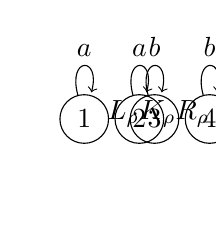
\begin{tikzpicture}[baseline=-10mm]
    \graphbox{$L_\rho$}{0mm}{0mm}{31mm}{20mm}{2mm}{-13mm}{
      \node [draw, circle] (x) at (-7mm,0mm) {1};
      \node [draw, circle] (y) at (0mm,0mm) {2};
      \draw[->] (x) edge[loop above] node  {$a$} (x);
      \draw[->] (y) edge [loop above] node {$a$} (y);
    }
    \graphbox{$K_\rho$}{32mm}{-0mm}{18mm}{20mm}{0mm}{-10mm}{
    }
    \begin{scope}[opacity=1]        
    \graphbox{$R_\rho$}{51mm}{-0mm}{38mm}{20mm}{2mm}{-13mm}{
      \node [draw, circle] (x) at (-7mm,0mm) {3};
      \node [draw, circle] (y) at (0mm,0mm) {4};
      \node [draw, circle] (z) at (7mm,0mm) {5};
      \draw[->] (x) edge[loop above] node  {$b$} (x);
      \draw[->] (y) edge[loop above] node  {$b$} (y);
      \draw[->] (z) edge[loop above] node  {$b$} (z);
    }
    \end{scope}
\end{tikzpicture}
}}
    \end{center}
    \begin{center}
    $\tau = $\scalebox{0.7}{ {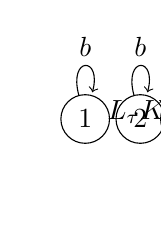
\begin{tikzpicture}[baseline=-10mm]
    \graphbox{$L_\tau$}{0mm}{0}{31mm}{20mm}{2mm}{-13mm}{
        \node[draw,circle] (x) at (-7mm,0mm) {1};
        \node[draw,circle] (y) at (0mm,0mm) {2};
        \draw[->] (x) edge[loop above] node {$b$} (x);
        \draw[->] (y) edge [loop above] node {$b$} (y);
      }
      \graphbox{$K_\tau$}{32mm}{0}{18mm}{20mm}{2mm}{-13mm}{
      }
      \begin{scope}[opacity=1]        
      \graphbox{$R_\tau$}{51mm}{0}{25mm}{20mm}{1mm}{-13mm}{
        \node[draw,circle] (x) at (-3.5mm,0mm) {3};
        \draw[->] (x) edge[loop above] node {$a$} (x);
      }
      \end{scope}
  \end{tikzpicture}}
    }
    \end{center}
     Let $X$ be the ruler-graph
    \tikz[baseline=-0.5ex]{
        \node (x) at (0,0) {$\bullet$};   
        \draw[->] (x) edge [loop right] node {a} (x);
    }, $Y$ the ruler-graph
    \tikz[baseline=-0.5ex]{
        \node (x) at (0,0) {$\bullet$};
        \draw[->] (x) edge [loop right] node {b} (x);
    } and $\mathbb{X} = \{X, Y\}$.
    The sets $D(R_\rho, X)$, $D(R_\rho, Y)$, $D(R_\tau, X)$ and $D(R_\tau, Y)$ are all empty. Therefore, both rules $\rho$ and $\tau$ are $X$- and $Y$-non-increasing because all conditions in \autoref{def:creates_more_x_on_the_left} are trivially satisfied.
    
    For $s_\mathbb{X}(X) = 5$ and $s_\mathbb{X}(Y) = 3$, we have $
    w_{s_\mathbb{X}}(L_\rho) = 10 > 9 = w_{s_\mathbb{X}}(R_\rho)
    $ and $
    w_{s_\mathbb{X}}(L_\tau) = 6 > 5 = w_{s_\mathbb{X}}(R_\tau)$.
    Thus, the system terminates by \autoref{thm:termination_grs}.

  However, for $s_\mathbb{X}'(X) = 1$ and $s_\mathbb{X}'(Y) = 1$, we have
    \(
        w_{s_\mathbb{X}'}(L_\rho) = 2 \not > 3 = w_{s_\mathbb{X}'}(R_\rho)
    \) which prevents us from applying \autoref{thm:termination_grs} to prove termination of the rewriting system.
    
\end{example}

% \begin{example}[Limitation]
%     \label{ex:plump95_4d1}
%    Consider a rule presented in \cite[Example 4.1]{Plump1995}:
 
%     \begin{center}
%         \resizebox{0.7\textwidth}{!}{
%       $\rho = $  \begin{tikzpicture}[baseline=-20mm]
%         \graphbox{$L$}{0mm}{0}{32mm}{40mm}{0}{0}{
%             \node[draw,circle]  (n1) at (0,-6mm) {1};
%             \node[draw,circle]   (n2) at (0mm,-26mm) {2};
%             \node[draw,circle]   (n3) at (-10mm,-26mm) {3};
%             \node[draw,circle]   (n4) at (10mm,-26mm) {4};
%             \draw[->]  (n2) edge [loop below] node  {a} (n2);
%             \draw[->]  (n3) edge [loop below] node  {b} (n3);
%             \draw[->]  (n1) to node [right] {f} (n2) ;
%             \draw[->]  (n1) to node [right] {f}  (n3);
%             \draw[->]  (n1) to node [right] {f}  (n4);
%           }
%           \graphbox{$K$}{33mm}{0}{32mm}{40mm}{0}{-0}{
%             \node[draw,circle]  (n1) at (0,-6mm) {1};
%             \node[draw,circle]   (n2) at (0mm,-26mm) {2};
%             \node[draw,circle]   (n3) at (-10mm,-26mm) {3};
%             \node[draw,circle]   (n4) at (10mm,-26mm) {4};
%             \draw[->]  (n2) edge [loop below] node  {a} (n2);
%             \draw[->]  (n3) edge [loop below] node  {b} (n3);
%           }
%           \graphbox{$R$}{66mm}{0}{32mm}{40mm}{0}{-0}{
%             \node[draw,circle]  (n1) at (0,-6mm) {1};
%             \node[draw,circle]   (n2) at (0mm,-26mm) {2};
%             \node[draw,circle]   (n3) at (-10mm,-26mm) {3};
%             \node[draw,circle]   (n4) at (10mm,-26mm) {4};
%             \draw[->]  (n2) edge [loop below] node  {a} (n2);
%             \draw[->]  (n3) edge [loop below] node  {b} (n3);
%             \draw[->]  (n1) edge [bend left] node [right] {f} (n4) ;
%             \draw[->]  (n1) edge [bend right] node [left] {f}  (n4);
%             \draw[->]  (n1) to node [right] {f}  (n4);
%           }   
%     \end{tikzpicture}
%         }
%   \end{center}
%   \noindent
%   \begin{minipage}{0.7\textwidth}
%     To prove its termination with our method, a ruler-graph $X$ containing an edge labeled by $f$ must be used, because the number of occurrences of every graph containing only edges labeled by $a$ and $b$ does not change by any rewriting step using $\rho$. But in this case, condition \eqref{def:non_increasing:edge_injective} of \autoref{def:creates_more_x_on_the_left} cannot be satisfied.
%   \end{minipage}
%   \begin{minipage}{0.3\textwidth}
%     \hfill
%   \begin{center}
%     \begin{tikzpicture} 
%         \graphbox{}{0}{0}{30mm}{20mm}{-10mm}{-10mm}{
%             \node[draw,circle]  (n1) at (0,0mm) {1};
%             % \node[draw,circle]   (n2) at (0mm,-26mm) {2};
%             % \node[draw,circle]   (n3) at (-10mm,-26mm) {3};
%             \node[draw,circle]   (n4) at (20mm,0mm) {4};
%             % \draw[->]  (n2) edge [loop below] node  {a} (n2);
%             % \draw[->]  (n3) edge [loop below] node  {b} (n3);
%             \draw[->]  (n1) edge [bend left] node [above] {f} (n4) ;
%             \draw[->]  (n1) edge [bend right] node [below] {f}  (n4);
%             \draw[->]  (n1) to node {f}  (n4);
%           }  
%     \end{tikzpicture}
%   \end{center}
% \end{minipage}
  
%   \end{example} 
% Finally, we present a limitation of our approach.
\begin{example}[Limitation]
    \label{rem:d3:limitation}  
    Our method fails to prove termination for the rewriting rule in \cite[Example D.3]{endrullis2024generalized}.
    % because our approach cannot take into account antipatterns(see~\cite[Remark 6.2]{overbeek2024termination_lmcs}).
    This failure occurs because, for any system $\mathcal{R}$, rewriting step $G \Rightarrow_{\mathcal{R},\mathfrak{M}} H$, set of ruler-graphs $\mathbb{X}$, and weight function $s_\mathbb{X}$, we have $w_{s_\mathbb{X}}(G) \geq w_{s_\mathbb{X}}(H)$ due to the existence of an injective graph homomorphism from $G$ to $H$.
    
    \begin{center}
        \resizebox{0.7\textwidth}{!}{
    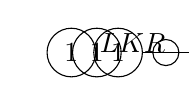
\begin{tikzpicture}  
       \graphbox{$L$}{0mm}{-11mm}{32mm}{15mm}{2mm}{-8mm}{  
           \node[draw,circle]  (x) at (-6mm,0mm) {1};  
           \node[draw,circle]  (y) at (6mm,0mm) {};  
         }  
         \graphbox{$K$}{33mm}{-11mm}{32mm}{15mm}{2mm}{-8mm}{  
           \node[draw,circle]  (x) at (-6mm,0mm) {1};  
         }  
         \graphbox{$R$}{66mm}{-11mm}{32mm}{15mm}{1mm}{-8mm}{  
          \node[draw,circle]  (x) at (-6mm,0mm) {1};  
          \node[draw,circle]  (y) at (6mm,0mm) {};  
          \draw[->]  (x) to (y);  
         }    
   \end{tikzpicture}
        }  
    \end{center}
  \end{example} 